%%%%%%%%%%%%%%%%%%%%%%%%%%%%%%%%%%%%%%%%%
% Jacobs Landscape Poster
% LaTeX Template
% Version 1.0 (29/03/13)
%
% Created by:
% Computational Physics and Biophysics Group, Jacobs University
% https://teamwork.jacobs-university.de:8443/confluence/display/CoPandBiG/LaTeX+Poster
% 
% Further modified by:
% Nathaniel Johnston (nathaniel@njohnston.ca)
%
% This template has been downloaded from:
% http://www.LaTeXTemplates.com
%
% 
% Masaryk University presentation themes were downloaded from:
% https://www.overleaf.com/gallery/tagged/muni
%
% and ported into Jacobs Landscape Poster by:
% Jumaidil Awal (ideal1st.here@googlemail.com)
% 
% Jacobs Landscape Poster License:
% CC BY-NC-SA 3.0 (http://creativecommons.org/licenses/by-nc-sa/3.0/)
%
% Masaryk University's fibeamer theme license:
% Copyright 2015  Vít Novotný <witiko@mail.muni.cz>
% Faculty of Informatics, Masaryk University (Brno, Czech Republic)
% under Latex Project Public License
%
%%%%%%%%%%%%%%%%%%%%%%%%%%%%%%%%%%%%%%%%%

%----------------------------------------------------------------------------------------
%	PACKAGES AND OTHER DOCUMENT CONFIGURATIONS
%----------------------------------------------------------------------------------------

\documentclass[final]{beamer}

\usepackage[scale=1]{beamerposter} % Use the beamerposter package for laying out the poster 1.24
\usepackage[style=numeric]{biblatex}
\addbibresource{sample.bib}

%\usetheme{confposter} % Use the confposter theme supplied with this template
\usetheme[faculty=chemo]{fibeamer} % Uncomment to use Masaryk University's fibeamer theme instead.

%\setbeamercolor{block title}{fg=ngreen,bg=white} % Colors of the block titles
%\setbeamercolor{block body}{fg=black,bg=white} % Colors of the body of blocks
%\setbeamercolor{block alerted title}{fg=white,bg=dblue!70} % Colors of the highlighted block titles
%\setbeamercolor{block alerted body}{fg=black,bg=dblue!10} % Colors of the body of highlighted blocks
% Many more colors are available for use in beamerthemeconfposter.sty

%-----------------------------------------------------------
% Define the column widths and overall poster size
% To set effective sepwid, onecolwid and twocolwid values, first choose how many columns you want and how much separation you want between columns
% In this template, the separation width chosen is 0.024 of the paper width and a 4-column layout
% onecolwid should therefore be (1-(# of columns+1)*sepwid)/# of columns e.g. (1-(4+1)*0.024)/4 = 0.22
% Set twocolwid to be (2*onecolwid)+sepwid = 0.464
% Set threecolwid to be (3*onecolwid)+2*sepwid = 0.708

\newlength{\sepwid}
\newlength{\onecolwid}
\newlength{\twocolwid}
\newlength{\threecolwid}
\setlength{\paperwidth}{46.8in} % A3 width: 46.8in
\setlength{\paperheight}{33.1in} % A3 height: 33.1in
\setlength{\sepwid}{0.024\paperwidth} % Separation width (white space) between columns 0.024
\setlength{\onecolwid}{0.21\paperwidth} % Width of one column 0.21
\setlength{\twocolwid}{0.451\paperwidth} % Width of two columns 0.451
\setlength{\threecolwid}{0.678\paperwidth} % Width of three columns 0.678
%\setlength{\topmargin}{-0.5in} % Reduce the top margin size
%-----------------------------------------------------------

\usepackage{graphicx}  % Required for including images

\usepackage{booktabs} % Top and bottom rules for tables

%----------------------------------------------------------------------------------------
%	TITLE SECTION 
%----------------------------------------------------------------------------------------

\title{The Baumgartner Jump} % Poster title

\author{Ruhan Ahmed, Jack Mortimer, Maya Tetteh, Saif-Ullah Hussain, Yuxin Ren} % Author(s)

\institute{University of Birmingham} % Institution(s)

%----------------------------------------------------------------------------------------

\begin{document}
\addtobeamertemplate{block end}{}{\vspace*{2ex}} % White space under blocks
\addtobeamertemplate{block example end}{}{\vspace*{2ex}} % White space under example blocks
\addtobeamertemplate{block alerted end}{}{\vspace*{2ex}} % White space under highlighted (alert) blocks

\setlength{\belowcaptionskip}{2ex} % White space under figures
\setlength\belowdisplayshortskip{2ex} % White space under equations
%\begin{darkframes} % Uncomment for dark theme, don't forget to \end{darkframes}
\begin{frame} % The whole poster is enclosed in one beamer frame

%==========================Begin Head===============================

  \begin{columns}
   \begin{column}{\linewidth}
    \vskip1cm
    \centering
    \usebeamercolor{title in headline}{\color{fg}\Huge{\textbf{\inserttitle}}\\[0.5ex]}
    \usebeamercolor{author in headline}{\color{fg}\Large{\insertauthor}\\[1ex]}
    \usebeamercolor{institute in headline}{\color{fg}\large{\insertinstitute}\\[1ex]}
    \vskip1cm
   \end{column}
   \vspace{1cm}
  \end{columns}
 \vspace{1cm}

%==========================End Head===============================

\begin{columns}[t] % The whole poster consists of three major columns, the second of which is split into two columns twice - the [t] option aligns each column's content to the top

\begin{column}{\sepwid}\end{column} % Empty spacer column

\begin{column}{\onecolwid} % The first column

%----------------------------------------------------------------------------------------
%	OBJECTIVES
%----------------------------------------------------------------------------------------

\begin{exampleblock}{Introduction}

The Baumgartner jump, a.k.a. Red Bull Stratos was a high-altitude diving project, in which the Austrian skydiver Felix Baumgartner jumped in free-fall, 39km above the Earth's surface. By generating an equation using constants such as mass, air density and the drag coefficient - we can predict the time and altitude when Felix reaches terminal velocity at, as well as predicting what velocity he travels when deploying the parachute

\end{exampleblock}

%----------------------------------------------------------------------------------------
%	INTRODUCTION
%----------------------------------------------------------------------------------------

\begin{exampleblock}{Assumptions}
\begin{itemize}
\item The value for acceleration due to gravity is constant at $g = 9.81\;m/s^2$. The Earth's radius is approximately 6,371 km and the height that Felix jumped from was 39 km above the surface; 163 times smaller than the Earth's radius, which would calculate to the acceleration due to gravity being negligible.\cite{Sharp}.

\item Felix's surface area, moving through the atmosphere, is constant during the free fall section of the jump and that he is falling vertically down. We have chosen to model the jump this way for simpler calculations, even though during the jump it was shown that he was rotating whilst falling.

\item The parachute deploys instantly, so that the increase in drag forces caused by the parachute opening also impacts the jump instantly. This also helps for simpler calculations in modelling the jump.

\item The air density is constant, in intervals of 10 km, from the jump's initial altitude to the Earth's surface. Since air density does affect the terminal velocity of a moving object \cite{Density}, we decided to use an average in intervals of 10km
\end{itemize}

\begin{center}
    
\includegraphics[scale=0.5]{img/Red_Bull_Stratos_logo.png}
\end{center}

\end{exampleblock}

%------------------------------------------------

\end{column} % End of the first column

\begin{column}{\sepwid}\end{column} % Empty spacer column

\begin{column}{\twocolwid} % Begin a column which is two columns wide (column 2)

\begin{columns}[t,totalwidth=\twocolwid] % Split up the two columns wide column

\begin{column}{\onecolwid}\vspace{-.74in} % The first column within column 2 (column 2.1)

%----------------------------------------------------------------------------------------
%	MATERIALS
%----------------------------------------------------------------------------------------

\begin{exampleblock}{Mathematical Section}

When Felix opens the parachute, the air resistance force increases - so the resultant force acts against the gravitational pull of the Earth, and thus Felix's velocity decreases. The acceleration of the jump can be modelled using the following equation, where:
\par $V$ is Felix's velocity
\par $t$ is time
\par $g$ is acceleration due to gravity
\par $\rho$ is air density
\par $C_d$ is the drag coefficient
\par $A$ is Felix's surface area

$$\frac{dv}{dt} = g - \frac{\rho C_d A}{2m}$$

\par By re-arranging variables and integrating with respect to time, we can find an equation for velocity and displacement:

$$V = \sqrt{\frac{2mg}{\rho C_d A}}\cdot\tanh{\left(\sqrt{\frac{\rho C_d A g}{2m}}t\right)}$$

$$S = \frac{2m}{\rho C_d A}\cdot\ln{\cosh{\left(\sqrt{\frac{\rho C_d A g}{2m}}t\right)}}$$

\par Where $S$ is Felix's displacement.
\par When his velocity decreases, the air resistance force also decreases in magnitude, until he reaches terminal velocity.
\newline
\begin{figure}
    \centering
    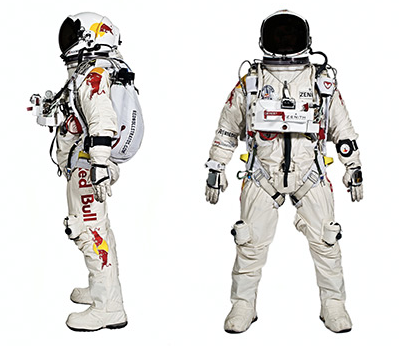
\includegraphics[scale=2.0]{img/baumgartner_suit.PNG}
    \caption{The Baumgartner Suit}
    \label{fig:my_label}
\end{figure}
 
\end{exampleblock}
%----------------------------------------------------------------------------------------

\end{column} % End of column 2.1
\begin{column}{\sepwid}\end{column} % Empty spacer column

\begin{column}{\onecolwid}\vspace{-.74in} % The second column within column 2 (column 2.2)

%----------------------------------------------------------------------------------------
%	METHODS
%----------------------------------------------------------------------------------------

\begin{exampleblock}{Graphs}
\begin{figure}
    \centering
    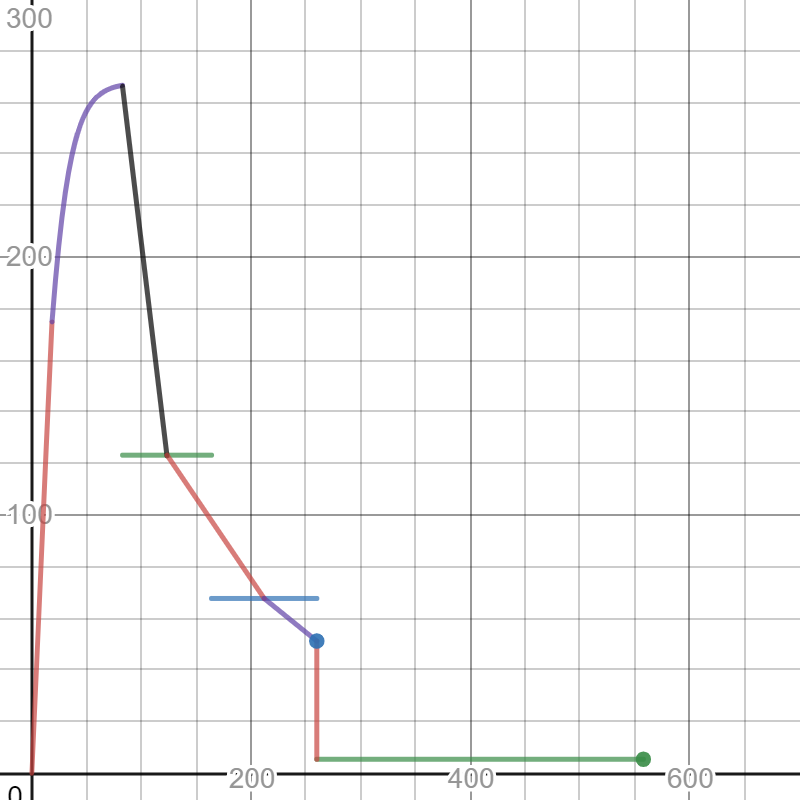
\includegraphics[width=1.0\linewidth]{img/velocity_graph.png}
    \caption{Velocity ($metres\;per\;second$) against time ($seconds$) graph}
    \label{fig:velocity}
\end{figure}
\begin{figure}
    \centering
    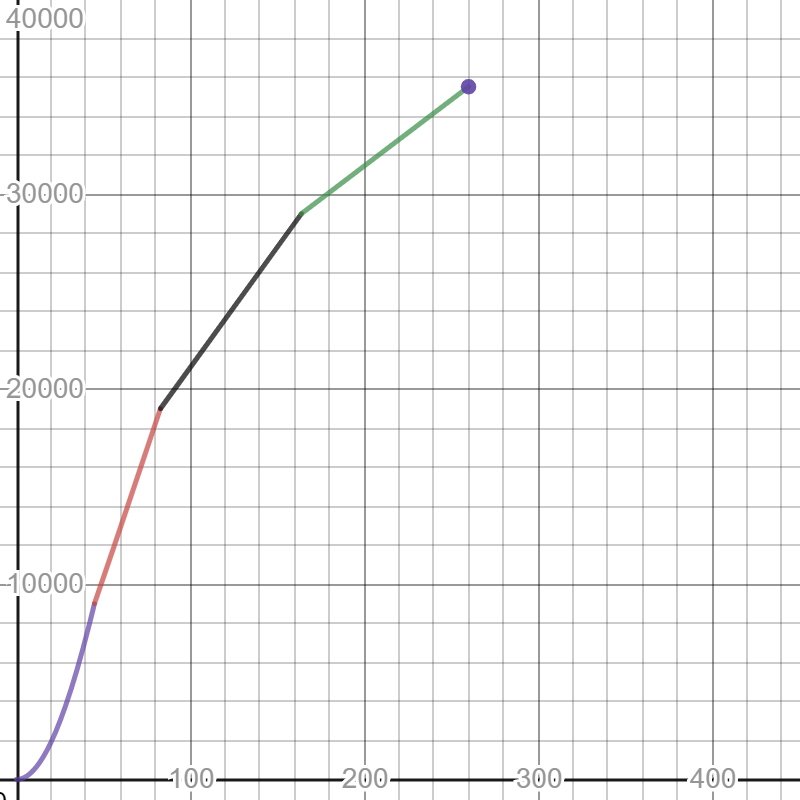
\includegraphics[width=1.0\linewidth]{img/displacement_graph.png}
    \caption{Displacement ($metres$) against time ($seconds$) graph}
    \label{fig:displacement}
\end{figure}
\end{exampleblock}



%------------------------

\end{column} % End of column 2.2

\end{columns} % End of the split of column 2 - any content after this will now take up 2 columns width



%----------------------------------------------------------------------------------------

\begin{columns}[t,totalwidth=\twocolwid] % Split up the two columns wide column again

\begin{column}{\onecolwid} % The first column within column 2 (column 2.1)

%----------------------------------------------------------------------------------------
%	MATHEMATICAL SECTION
%----------------------------------------------------------------------------------------




%----------------------------------------------------------------------------------------

\end{column} % End of column 2.1
\begin{column}{\sepwid}\end{column} % Empty spacer column

\begin{column}{\onecolwid} % The second column within column 2 (column 2.2)


%----------------------------------------------------------------------------------------

\end{column} % End of column 2.2

\end{columns} % End of the split of column 2

\end{column} % End of the second column

\begin{column}{\sepwid}\end{column} % Empty spacer column

\begin{column}{\onecolwid} % The third column

%----------------------------------------------------------------------------------------
%	CONCLUSION
%----------------------------------------------------------------------------------------

\begin{exampleblock}{Graph results}

The different coloured sections on each graph represent each interval of altitude, chosen for each mean air density. In the graph of velocity against time, the velocity reaches its maximum at \textbf{83 seconds}.\par However, at greater densities of air the further Felix falls, the graph of each section suggests that such a velocity would never have been reached. This indicates the velocity would decrease after reaching its maximum. When Felix opens his parachute at \textbf{260\textit{s}}, his velocity decreases substantially - from \textbf{51.2\textit{m/s}} to \textbf{5.4\textit{m/s}} - and remains relatively constant until he reaches the ground at \textbf{558 seconds}.

It has been assumed that velocity would decrease linearly between each mean density of air and that the mean density of air occurs in the middle of the interval. It is then assumed that at the time Felix opens his parachute, his velocity decreases instantly to the limit of velocity he would experience if he had his parachute open, as a rapid decrease in velocity would be expected.


He opens his parachute at 260s as stated at a velocity of approx 51.2 mps and altitude of 3496m

He reaches the ground at 558s as in reality (found from the real mission data) at a velocity of approx. 5.4 mps

His max velocity is about 267mps at 83s

\end{exampleblock}

%----------------------------------------------------------------------------------------
%	ADDITIONAL INFORMATION
%----------------------------------------------------------------------------------------

\begin{exampleblock}{Red Bull Stratos Data}

Maecenas ultricies feugiat velit non mattis. Fusce tempus arcu id ligula varius dictum. 
\begin{itemize}
\item Curabitur pellentesque dignissim
\item Eu facilisis est tempus quis
\item Duis porta consequat lorem
\item Duis porta consequat lorem
\end{itemize}

\end{exampleblock}

%----------------------------------------------------------------------------------------
%	REFERENCES
%----------------------------------------------------------------------------------------

\begin{exampleblock}{Refinements}
SDIUFHSDIFHklsDHFilSHFISEHUBGIBDFKGHZDKFG HJoifhgo;zidhfgo
\end{exampleblock}

\begin{exampleblock}{References}
    \printbibliography
\end{exampleblock}




%----------------------------------------------------------------------------------------

\end{column} % End of the third column

\begin{column}{\sepwid}\end{column} % Empty spacer column

\end{columns} % End of all the columns in the poster

\end{frame} % End of the enclosing frame
%\end{darkframes} % Uncomment for dark theme
\end{document}
